\documentclass[12pt, a4paper]{report}

\usepackage{inputenc}
\usepackage[spanish]{babel}
\usepackage{graphicx}
%\usepackage{fontspec}
%\usepackage{classicthesis} 
%\usepackage{arsclassica}
\usepackage[hidelinks]{hyperref}
%\usepackage{bookmark}
\usepackage[table]{xcolor}
\usepackage{parskip}
\usepackage{float}
\usepackage{listings}
\usepackage{apacite}
\usepackage{pdfpages}

\begin{document}
\includepdf[pages={1}]{../Attachments/PortadaResumen.pdf}

\chapter{Introducci\'on}
El Trabajo de Fin de Grado (a partir de ahora TFG) aqu\'{i} presentado fue 
propuesto por un profesor de la universidad. Las razones de la aceptaci\'{o}n 
del TFG fueron que se ve\'{i}a una continuidad, es decir, que se pod\'{i}a 
utilizar el TFG como entrada a un grupo de investigaci\'{o}n y/o continuar con 
el trabajo durante un m\'{a}ster.

El software ha sido liberado bajo licencia GPLv3 o posterior, y puede 
encontrarse en \url{https://github.com/RubenAgudo/MIPS}.

\chapter{Objetivos del proyecto}
\section{Objetivos}
Los objetivos del proyecto consisten en crear un software que extienda la 
funcionalidad actual del sistema ULISES desarrollado 
por la universidad de Navarra y del grupo de investigación GALAN perteneciente 
a la UPV/EHU.

El software, debe permitir cargar observaciones y propiedades previamente 
capturadas con diversos
sistemas interactivos (por ejemplo, con un dispositivo Kinect) y
visualizarlas gr\'aficamente. Esas observaciones y propiedades se cargar\'an en 
un panel lateral con forma de \'arbol
y podr\'an seleccionarse para ser visualizadas. Los gr\'aficos pueden ser 
reorganizados como el
usuario quiera, para verlos al mismo tiempo.

\chapter{Antecedentes}
\section{Situaci\'on actual}
El proyecto ULISES desarrollado por el grupo de investigaci\'on GaLan, en 
colaboraci\'on con la universidad de Navarra, consiste en un software que 
permite la integraci\'on de cualquier sistema interactivo con cualquier sistema 
educativo. Es decir, sirve para ense\~nar habilidades que necesitan de un 
profesor experto que los eval\'ue, ya sea en tiempo real, o a trav\'es de un 
v\'ideo.

\chapter{Captura de requisitos}
\section{Diagrama de casos de uso}
En el diagrama de casos de uso, se puede ver que acciones puede realizar el 
usuario en cualquier momento, y cuales
est\'an supeditadas a ciertas condiciones. N\'otese que las condiciones de los 
``extend" \ son los comentarios a\~nadidos
a los subcasos de uso.

\begin{figure}[h]
\centering
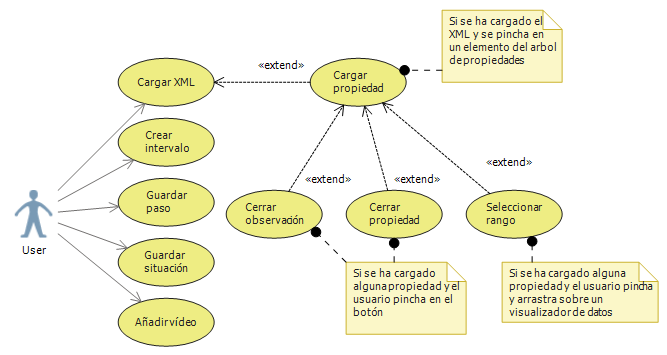
\includegraphics[width=1.0\linewidth]{../Figures/useCaseDiagram.png}
\caption[Diagrama de casos de uso]{Diagrama de casos de uso}
\label{fig:useCaseDiagram}
\end{figure}

\chapter{Analisis y dise\~no}
En este cap\'itulo se describen aquellas bibliotecas y patrones de dise\~no que 
se han usado. Tambi\'en se describe como han sido aplicadas en MIPS por ejemplo 
SOLID y los patrones MVVM, Iterator y el Clean Code.

\chapter{Desarrollo}
\section{Qu\'e se ha hecho}
Se ha desarrollado una aplicaci\'{o}n que dados unos datos organizados de 
cierta manera permite la visualizaci\'{o}n de los mismos y la selecci\'{o}n de 
unos rangos para guardar y especificar que en ese rango de tiempo est\'{a} 
sucediendo una acci\'{o}n determinada, ya sea un Paso o una Situaci\'on.

\chapter{Verificaci\'on y evaluaci\'on}
En este cap\'itulo se detallar\'an las pruebas
que se han llevado a cabo para verificar que el software
cumple todos los requisitos correctamente.

Las pruebas representan los comportamientos que debe
tener la aplicaci\'on, es decir, lo que se prueban son los
casos de uso y subcasos de uso, no si cada m\'etodo
realiza de forma correcta su tarea.

\chapter{Conclusiones y trabajo futuro}
Para finalizar, en una memoria no puede faltar una secci\'on en la cual el 
desarrollador hace una reflexi\'on sesuda sobre el trabajo realizado, qu\'e es 
lo que se planific\'o y lo que ha sido realmente...
\end{document}
